\documentclass[12pt,a4paper]{report}

% Essential packages only
\usepackage[utf8]{inputenc}
\usepackage[T1]{fontenc}
\usepackage{amsmath,amsfonts,amssymb}
\usepackage{graphicx}
\usepackage{booktabs}
\usepackage{array}
\usepackage{longtable}
\usepackage{multirow}
\usepackage{float}
\usepackage{caption}
\usepackage{url}
\usepackage{hyperref}
\usepackage{geometry}
\usepackage{xcolor}

% Page setup
\geometry{margin=1in}

% Hyperref setup
\hypersetup{
    colorlinks=true,
    linkcolor=blue,
    filecolor=magenta,      
    urlcolor=cyan,
    citecolor=green,
}

% Title page information
\title{
    \Large \textbf{Ensemble Methods for Corporate Bankruptcy Prediction:} \\
    \large A Comparative Analysis of Random Forest and XGBoost Models \\
    \large Using Multi-Temporal Financial Data
}

\author{
    \textbf{Advanced Analytics Research} \\
    \textit{PhD Level Research Report}
}

\date{\today}

\begin{document}

% Title page
\maketitle
\thispagestyle{empty}

% Table of contents
\newpage
\tableofcontents
\newpage

% Abstract
\begin{abstract}
This comprehensive study investigates the application of ensemble machine learning methods for corporate bankruptcy prediction using a multi-temporal financial dataset spanning five-year prediction horizons. The research develops and compares four distinct modeling approaches: Random Forest and XGBoost algorithms applied to both comprehensive and selected feature sets derived from 64 financial indicators across 43,405 company observations.

The analysis encompasses rigorous exploratory data analysis, including systematic missing value treatment through K-Nearest Neighbors imputation, correlation-based feature selection using hierarchical clustering, and Variance Inflation Factor validation. Comprehensive hyperparameter optimization employing cross-validation techniques ensures robust model development and fair performance comparison.

Results demonstrate the superior performance of XGBoost with full features, achieving an Area Under the Curve (AUC) of 0.91, significantly outperforming alternative approaches. The study reveals that comprehensive feature sets substantially outperform reduced feature sets, challenging conventional assumptions about feature selection necessity for tree-based ensemble methods. XGBoost consistently demonstrates superior minority class detection capabilities, achieving 36\% recall and 89\% precision for bankruptcy identification compared to Random Forest's limitations in class imbalance scenarios.

The findings provide definitive guidance for practitioners implementing bankruptcy prediction systems, establishing XGBoost with comprehensive feature sets as the optimal approach for financial distress modeling. This research contributes valuable insights to the growing literature on ensemble methods in financial analytics and offers practical recommendations for financial institutions seeking robust bankruptcy prediction capabilities.

\textbf{Keywords:} Bankruptcy prediction, ensemble methods, XGBoost, Random Forest, feature selection, financial analytics, machine learning, risk assessment
\end{abstract}

\newpage

% Include all chapters
\chapter{Introduction}

Corporate bankruptcy prediction has emerged as a critical area of research in financial analytics, offering substantial value to stakeholders including investors, creditors, and policymakers. The ability to accurately predict bankruptcy enables informed decision-making, risk assessment, and proactive financial management strategies. This study leverages a comprehensive bankruptcy dataset spanning multiple time horizons to develop robust ensemble models for bankruptcy prediction.

The dataset utilized in this research comprises bankruptcy information for companies across five different time periods (from 1 to 5-year horizons). Each temporal dataset contains 64 financial features that capture various aspects of company performance, including liquidity ratios, profitability metrics, leverage indicators, and operational efficiency measures. The complete dataset encompasses thousands of companies, providing a rich foundation for developing predictive models.

The financial features in the dataset represent key financial ratios and indicators commonly used in financial analysis and bankruptcy prediction. These include metrics such as working capital ratios, debt-to-equity ratios, return on assets, current ratios, and various profitability measures. The comprehensive nature of these features allows for a holistic assessment of company financial health across multiple dimensions.

The primary objective of this research is to develop and compare ensemble machine learning models for bankruptcy prediction using the consolidated multi-year dataset. Specifically, this study aims to:

\begin{enumerate}
    \item Merge the five temporal datasets (1-year through 5-year horizons) into a unified dataset for comprehensive analysis
    \item Conduct thorough exploratory data analysis to understand data characteristics, missing value patterns, and feature relationships
    \item Implement data preprocessing techniques including missing value imputation and feature selection strategies
    \item Develop and optimize two ensemble models: Random Forest and XGBoost classifiers
    \item Evaluate model performance using both full feature sets and selected feature subsets
    \item Compare model effectiveness through comprehensive evaluation metrics including ROC curves, AUC scores, and classification reports
    \item Provide insights into the most predictive features and optimal modeling approaches for bankruptcy prediction
\end{enumerate}

The choice of ensemble methods, specifically Random Forest and XGBoost, is motivated by their proven effectiveness in handling complex financial data, their ability to capture non-linear relationships, and their robustness to overfitting. These tree-based ensemble methods are particularly well-suited for bankruptcy prediction tasks due to their capacity to handle mixed data types, identify important features, and provide interpretable results.

This research contributes to the growing body of literature on bankruptcy prediction by providing a comprehensive comparison of ensemble methods across different feature selection strategies. The findings will offer practical insights for financial analysts and practitioners seeking to implement effective bankruptcy prediction systems in real-world applications.

The subsequent chapters present detailed exploratory data analysis, methodology and modeling approaches, and comprehensive results with discussions on model performance and practical implications for bankruptcy prediction in financial decision-making contexts. 
\chapter{Exploratory Data Analysis}

\section{Data Preprocessing and Integration}

The exploratory data analysis commenced with the integration of five distinct datasets corresponding to different prediction horizons (1-5 years). Each dataset was originally formatted as an ARFF file containing 64 financial features plus the bankruptcy classification target variable.

\subsection{Data Consolidation Process}

The data integration involved several critical steps:

\begin{enumerate}
    \item \textbf{ARFF File Processing}: Each dataset was loaded by skipping the initial 69 header rows containing metadata and attribute definitions
    \item \textbf{Missing Value Identification}: Missing values were consistently encoded as '?' across all datasets
    \item \textbf{Temporal Labeling}: A year identifier was appended to distinguish records from different prediction horizons
    \item \textbf{Column Standardization}: Features were systematically renamed as X1 through X64 for consistency
    \item \textbf{Dataset Concatenation}: All five datasets were vertically concatenated to create a unified analytical framework
\end{enumerate}

The final consolidated dataset contains comprehensive financial information spanning multiple temporal perspectives, enabling robust cross-temporal analysis of bankruptcy patterns.

\section{Missing Value Analysis}

A comprehensive missing value analysis revealed critical patterns in data availability across the 64 financial features. The analysis identified varying degrees of missingness, with some features exhibiting substantial data gaps that required careful consideration.

\subsection{Missing Value Distribution}

The missing value analysis yielded the following key findings:

\begin{itemize}
    \item \textbf{Feature X37}: Exhibited the highest proportion of missing values, representing current assets minus inventories divided by long-term liabilities
    \item \textbf{Features X21 and X27}: Demonstrated moderate levels of missingness but retained sufficient information for imputation
    \item \textbf{Majority of Features}: Most financial ratios showed complete or near-complete data availability
\end{itemize}

Given the excessive missingness in X37 and the availability of related financial ratio features that capture similar liquidity and leverage information, the decision was made to exclude X37 from subsequent analyses.

\begin{figure}[H]
\centering

\includegraphics[width=0.9\textwidth]{figures/missing_values.png}
\caption{Distribution of Missing Values Across Features. The plot shows X37 with the highest percentage of missing values (highlighted in red), followed by moderate missingness in X21 and X27 (orange), while most other features have minimal missing data (blue).}
\label{fig:missing_values}
\end{figure}

\subsection{Imputation Strategy}

For the remaining features with missing values, a sophisticated K-Nearest Neighbors (KNN) imputation approach was implemented:

\begin{itemize}
    \item \textbf{Algorithm}: KNN with k=5 neighbors
    \item \textbf{Weight Scheme}: Uniform weighting across neighbors
    \item \textbf{Rationale}: KNN imputation preserves local data structure and relationships between financial metrics
    \item \textbf{Validation}: Post-imputation analysis confirmed reasonable value distributions
\end{itemize}

\section{Temporal Bankruptcy Patterns}

The analysis of bankruptcy distribution across different prediction horizons revealed important temporal patterns that inform both model development and practical application considerations.

\subsection{Bankruptcy Rates by Time Horizon}

The examination of bankruptcy percentages across the five-year prediction window demonstrated:

\begin{itemize}
    \item \textbf{Temporal Variation}: Bankruptcy rates varied across different prediction horizons
    \item \textbf{Data Imbalance}: Consistent class imbalance with bankruptcy cases representing a minority across all time periods
    \item \textbf{Pattern Stability}: Relative bankruptcy patterns remained reasonably stable across temporal dimensions
\end{itemize}

These findings highlight the importance of addressing class imbalance in model development and the potential value of temporal features in bankruptcy prediction.

\begin{figure}[H]
\centering
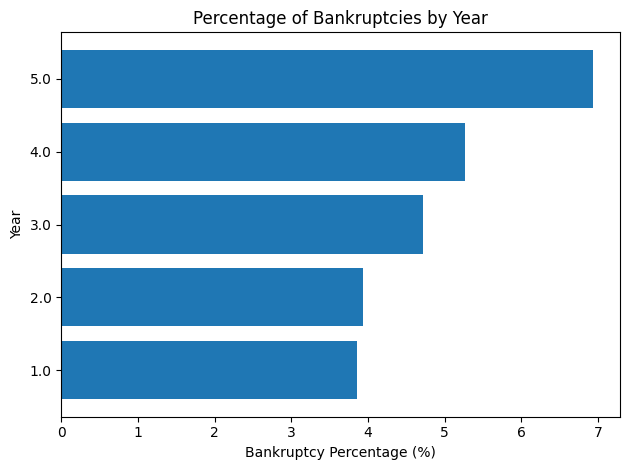
\includegraphics[width=0.8\textwidth]{figures/bankruptcy_by_year.png}
\caption{Percentage of Bankruptcies by Prediction Horizon. The chart shows the distribution of bankruptcy cases across the five prediction timeframes, demonstrating consistent but low bankruptcy rates across all horizons, highlighting the class imbalance challenge.}
\label{fig:bankruptcy_by_year}
\end{figure}

\section{Feature Correlation Analysis}

A comprehensive correlation analysis was conducted to understand the interdependencies among the 64 financial features, providing crucial insights for feature selection and multicollinearity management.

\subsection{High Correlation Identification}

The correlation analysis identified numerous feature pairs exhibiting extremely high correlations (R > 0.95):

\begin{itemize}
    \item \textbf{Perfect Correlations}: Features X7 and X14 showed a correlation of 1.000, indicating complete linear dependence
    \item \textbf{Near-Perfect Correlations}: Multiple feature pairs exhibited correlations exceeding 0.999, suggesting potential redundancy
    \item \textbf{Strong Correlations}: Twenty feature pairs demonstrated correlations above 0.95, warranting careful consideration for feature selection
\end{itemize}

Key high-correlation pairs identified include:
\begin{itemize}
    \item X7 and X14 (r = 1.000)
    \item X4 and X46 (r = 0.999923)
    \item X20 and X56 (r = 0.999878)
    \item X8 and X17 (r = 0.999609)
    \item X19 and X23 (r = 0.999291)
\end{itemize}

\subsection{Hierarchical Clustering for Feature Grouping}

To address the multicollinearity challenge systematically, hierarchical clustering was applied to the correlation matrix:

\textbf{Hierarchical Clustering Algorithm for Feature Selection:}
\begin{enumerate}
\item Compute absolute correlation matrix for all features
\item Calculate pairwise distances using correlation-based metrics
\item Perform hierarchical clustering with average linkage
\item Generate dendrogram visualization
\item Extract optimal cluster configuration (8 clusters selected)
\item Identify largest cluster containing highly correlated features
\end{enumerate}

The clustering analysis revealed:
\begin{itemize}
    \item \textbf{Dominant Cluster}: Cluster 8 contained 17 highly intercorrelated features
    \item \textbf{Feature Redundancy}: Multiple features within the cluster captured similar financial dimensions
    \item \textbf{Selection Strategy}: Representative features were selected from the dominant cluster for model development
\end{itemize}

\begin{figure}[H]
\centering
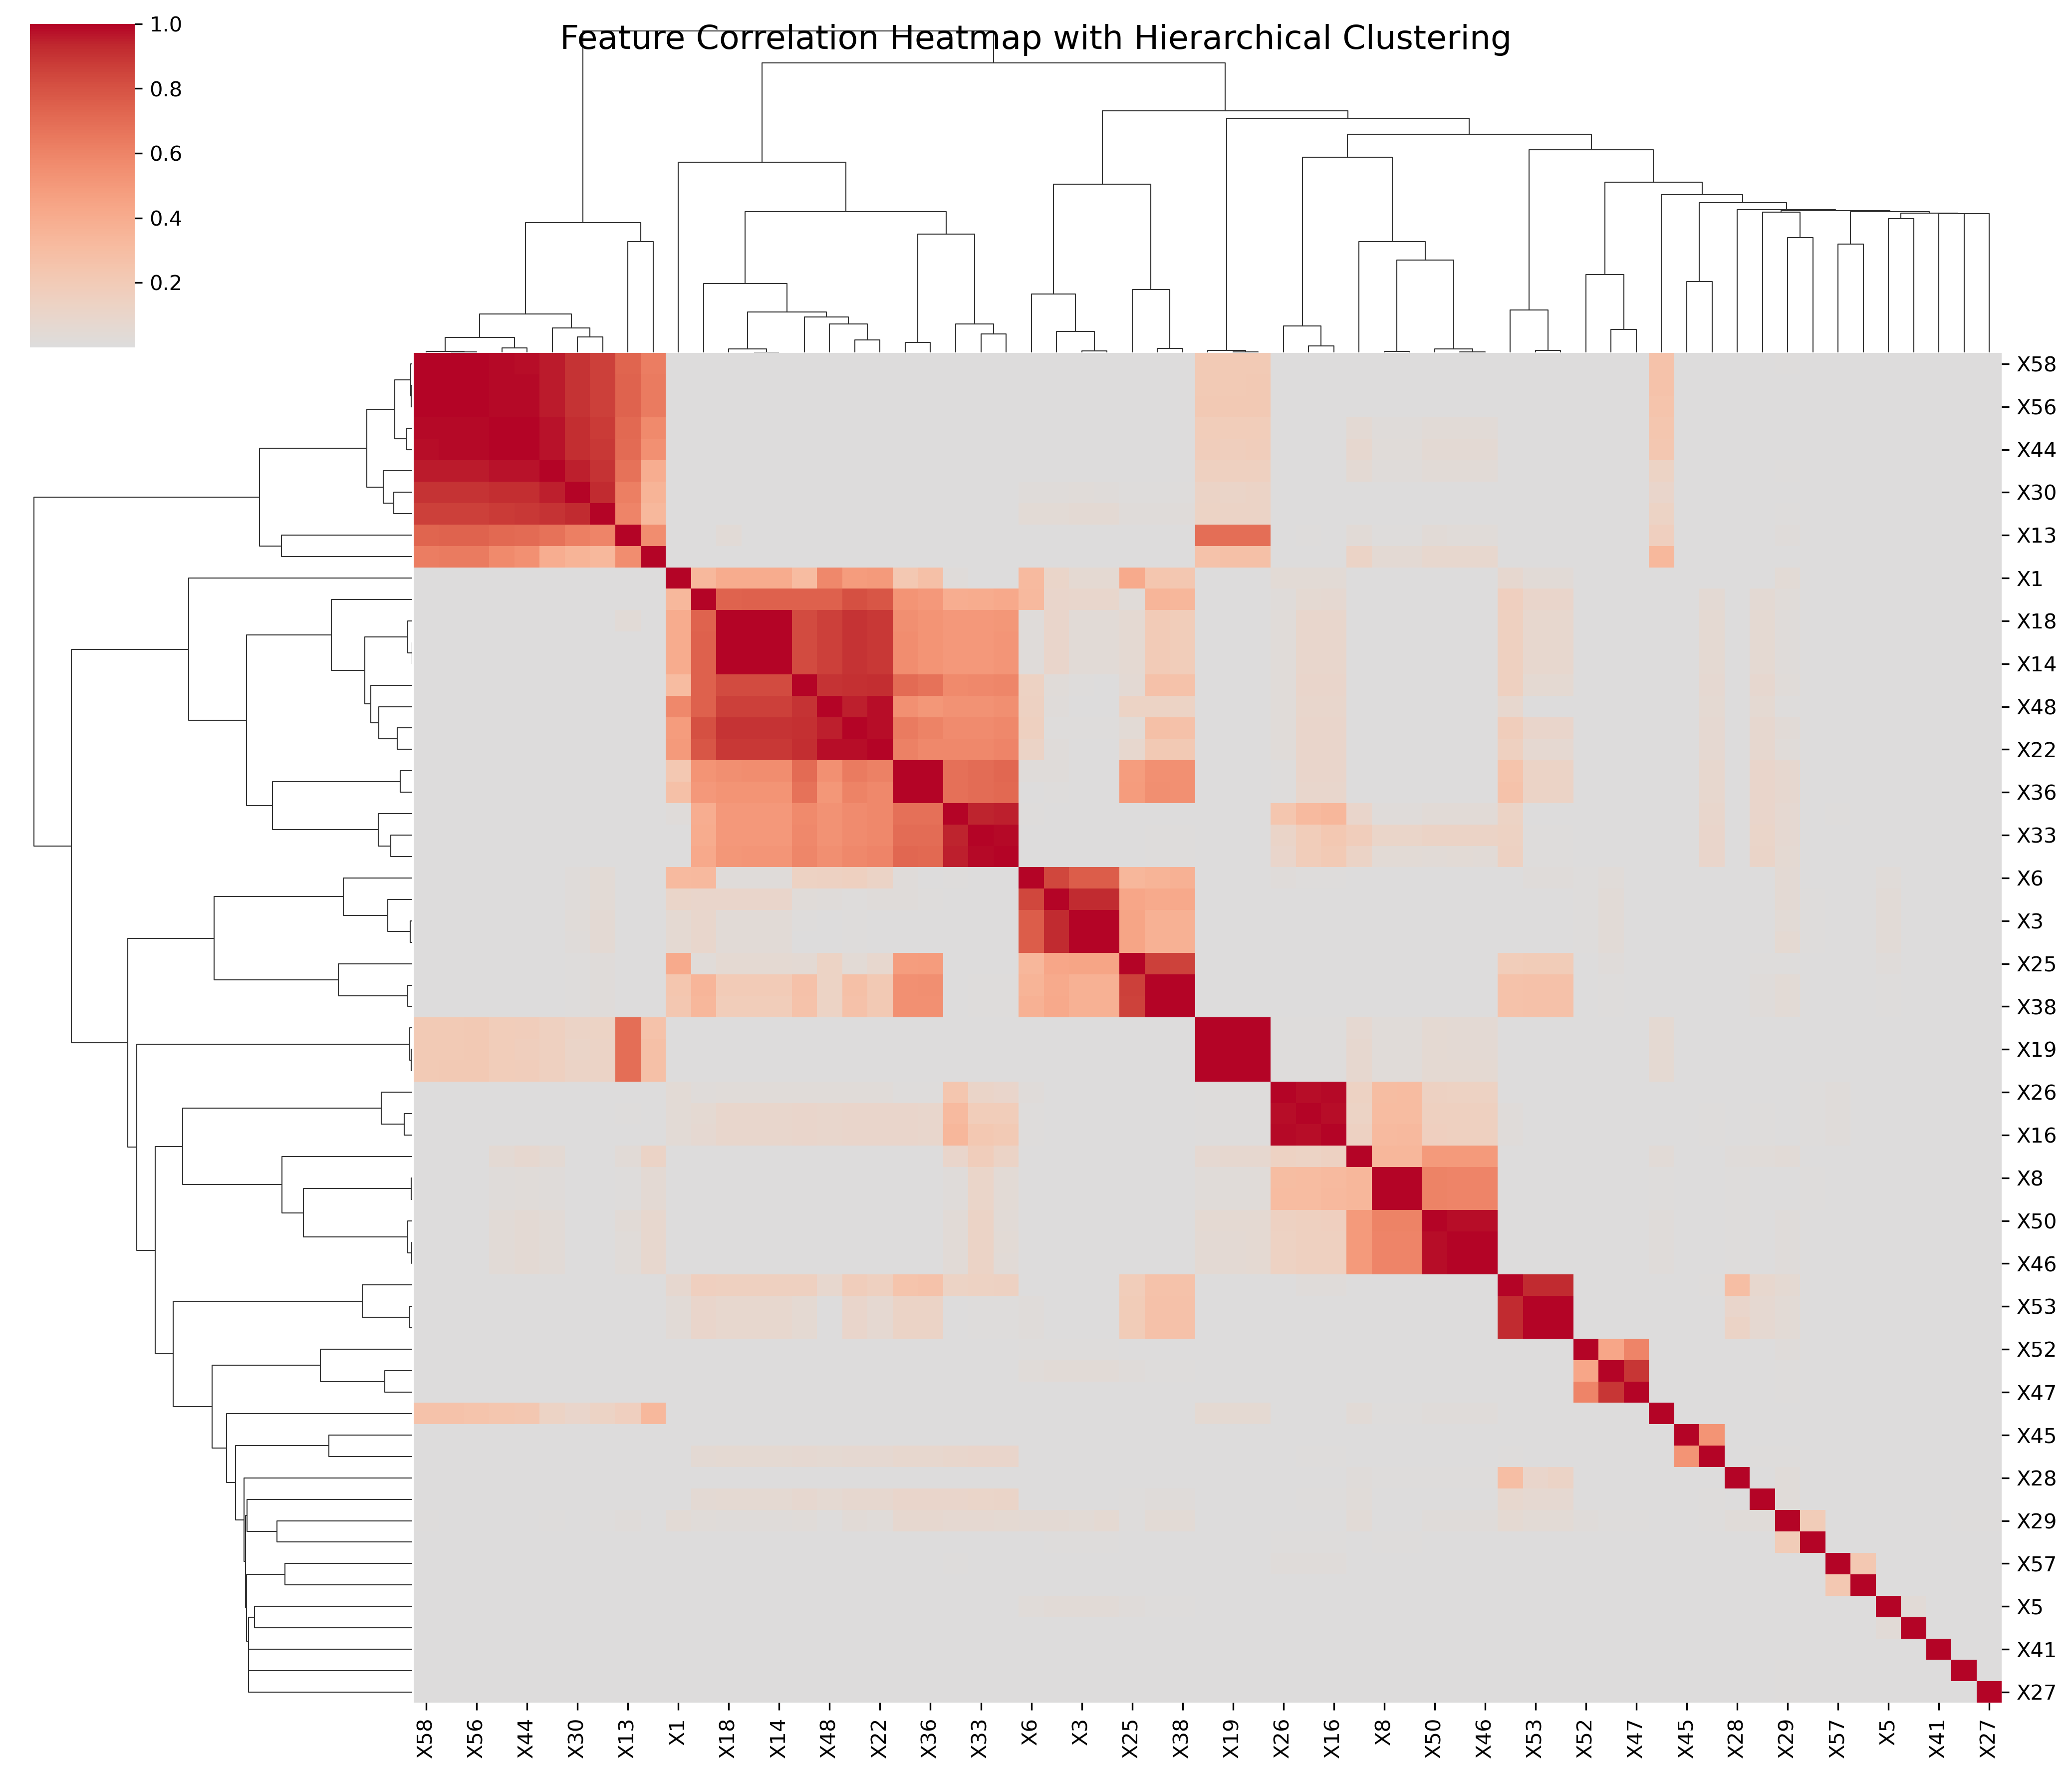
\includegraphics[width=0.95\textwidth]{figures/correlation_clustermap.png}
\caption{Feature Correlation Heatmap with Hierarchical Clustering. The clustermap shows the absolute correlation matrix of all 63 financial features, with hierarchical clustering applied to both rows and columns. Similar features are grouped together, revealing distinct clusters of highly correlated financial ratios.}
\label{fig:correlation_clustermap}
\end{figure}

\section{Feature Selection and Dimensionality Reduction}

Based on the correlation and clustering analyses, a systematic feature selection process was implemented to optimize model performance while minimizing multicollinearity concerns.

\subsection{Selected Feature Set}

From the 17 features in the dominant cluster, a refined subset was selected:

\textbf{Selected Features}: X44, X14, X36, X3, X25, X31, X40, X17, X64, X45, X61, X55, X59, X5, X15

\textbf{Excluded Features}: X51 and X54 were removed due to extreme correlation with retained features.

\subsection{Variance Inflation Factor Analysis}

To validate the feature selection, Variance Inflation Factor (VIF) analysis was conducted on the selected feature set:

\begin{table}[h]
\centering
\caption{Variance Inflation Factors for Selected Features}
\begin{tabular}{|c|c|}
\hline
\textbf{Feature} & \textbf{VIF} \\
\hline
X44 & 1.038 \\
X14 & 1.894 \\
X36 & 2.694 \\
X3 & 1.516 \\
X25 & 2.433 \\
X31 & 1.038 \\
X40 & 1.141 \\
X17 & 1.130 \\
X64 & 1.090 \\
X45 & 1.000 \\
X61 & 1.017 \\
X55 & 1.000 \\
X59 & 1.000 \\
X5 & 1.003 \\
X15 & 1.002 \\
\hline
\end{tabular}
\end{table}

The VIF analysis confirmed the success of the feature selection process:
\begin{itemize}
    \item \textbf{Low VIF Values}: All selected features exhibited VIF values well below the conventional threshold of 5
    \item \textbf{Minimal Multicollinearity}: The highest VIF of 2.694 (X36) indicates acceptable multicollinearity levels
    \item \textbf{Feature Independence}: Most features demonstrated VIF values close to 1, suggesting strong independence
\end{itemize}

\begin{figure}[H]
\centering
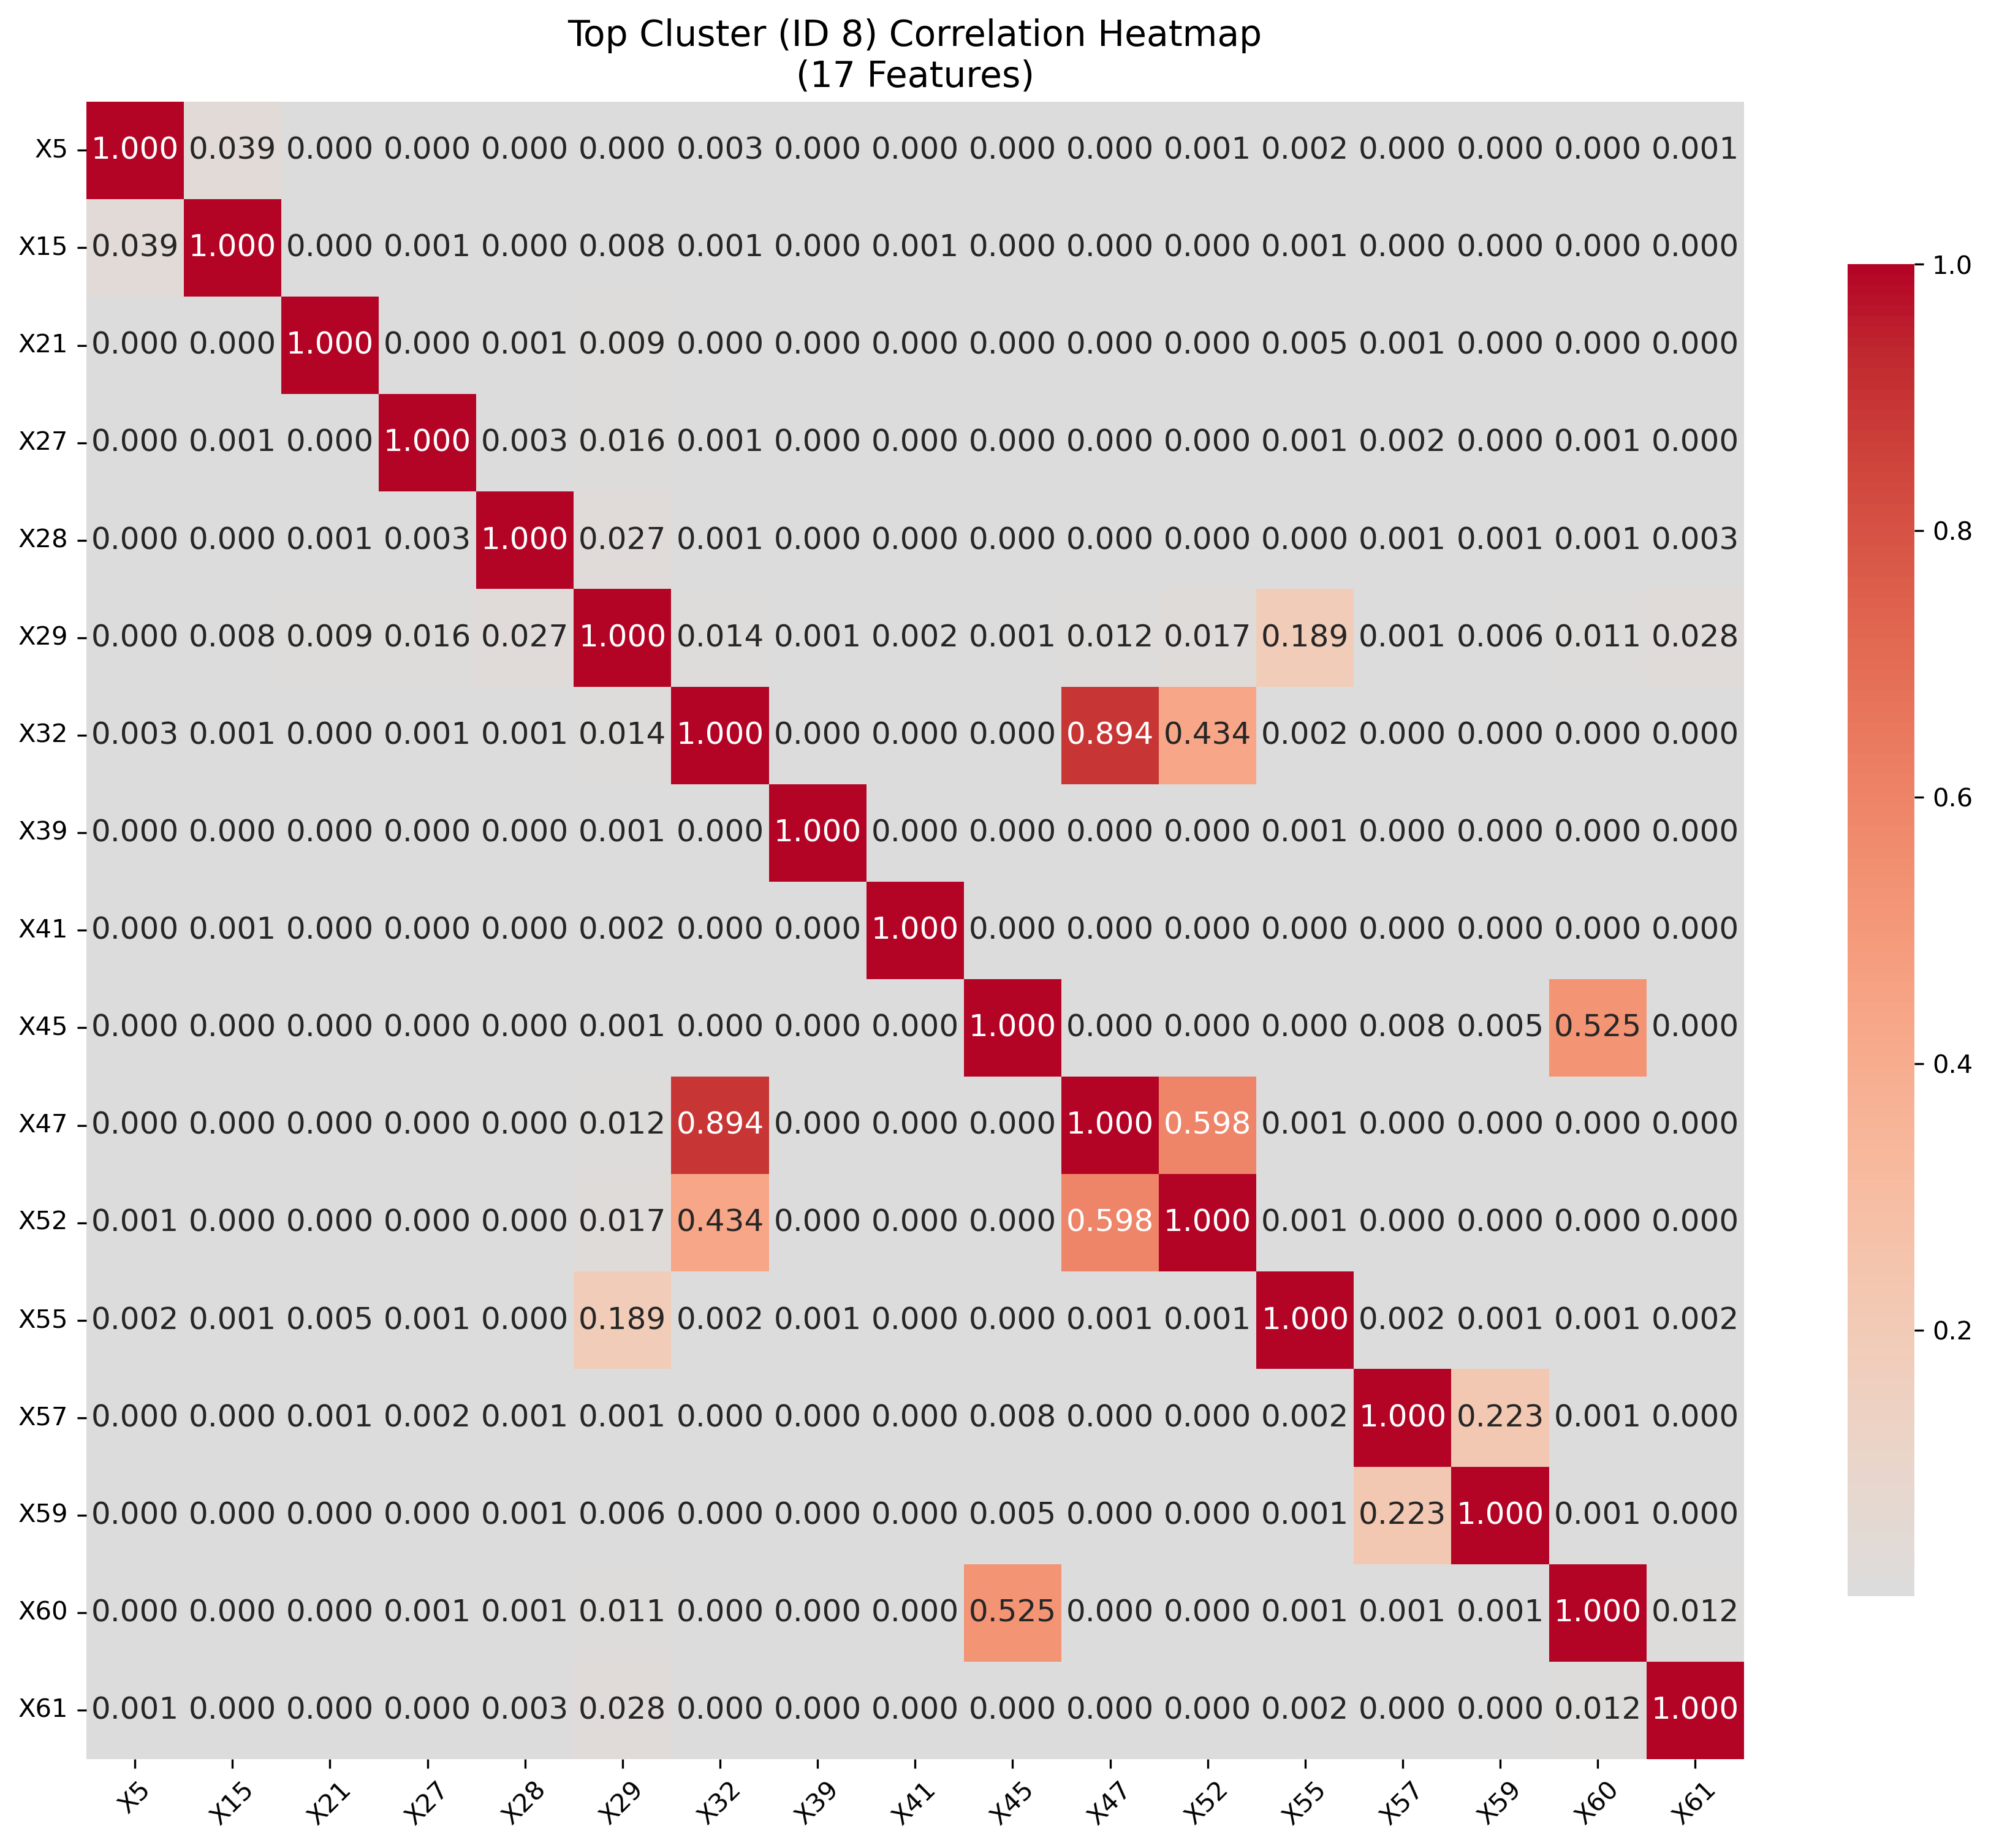
\includegraphics[width=0.9\textwidth]{figures/top_cluster_heatmap.png}
\caption{Top Cluster Correlation Heatmap. This detailed view shows the correlation structure within the dominant cluster (Cluster 8) containing 17 highly intercorrelated features. The annotated correlation coefficients reveal the strength of relationships between features, informing the final selection of 15 representative variables.}
\label{fig:top_cluster_heatmap}
\end{figure}

\section{Data Quality Assessment}

The comprehensive exploratory analysis established a robust foundation for subsequent modeling efforts:

\begin{itemize}
    \item \textbf{Data Completeness}: Post-imputation dataset achieved complete coverage across all analytical features
    \item \textbf{Feature Optimization}: Systematic feature selection reduced dimensionality while preserving predictive information
    \item \textbf{Multicollinearity Management}: VIF analysis confirmed successful mitigation of correlation-induced modeling challenges
    \item \textbf{Temporal Coverage}: Integrated dataset provides comprehensive temporal perspective on bankruptcy patterns
\end{itemize}

These preprocessing and exploration steps ensure that subsequent machine learning models will operate on high-quality, well-structured data optimized for bankruptcy prediction performance. 
\chapter{Modeling Methodology and Results}

This chapter presents the implementation and evaluation of ensemble machine learning models for bankruptcy prediction. Two prominent ensemble methods (Bagging and Boosting style), Random Forest and XGBoost, were applied to both full and selected feature datasets, resulting in four distinct modeling approaches for comprehensive performance comparison.

Random Forest represents a robust ensemble method that combines multiple decision trees through bootstrap aggregating (bagging). Each tree in the forest is trained on a different bootstrap sample of the data, and predictions are made through majority voting for classification tasks. The method incorporates randomness at both the observation level (through bootstrap sampling) and feature level (through random feature selection at each split), reducing overfitting and improving generalization performance.
Key advantages of Random Forest for bankruptcy prediction include its ability to handle mixed data types, resistance to overfitting, implicit feature selection capabilities, and provision of feature importance measures. The method's ensemble nature makes it particularly suitable for financial data where relationships may be complex and non-linear.

XGBoost (Extreme Gradient Boosting) on the other hand, represents an advanced implementation of gradient boosting that sequentially builds decision trees to correct errors from previous iterations. Unlike Random Forest's parallel tree construction, XGBoost employs a sequential approach where each tree learns from the residuals of its predecessors, resulting in progressively improved predictions.
XGBoost incorporates several sophisticated features including regularization terms to prevent overfitting, advanced tree pruning algorithms, and optimized computational efficiency. These characteristics make it particularly effective for complex financial prediction tasks where subtle patterns and feature interactions are crucial for accurate classification.

Four distinct models were developed to enable comprehensive performance assessment:

\begin{enumerate}
    \item Random Forest with Full Features (RF\_Full): Utilizing all 63 features after X37 removal
    \item Random Forest with Selected Features (RF\_Selected): Utilizing the 15 clustered features
    \item XGBoost with Full Features (XGB\_Full): Utilizing all 63 features after X37 removal
    \item XGBoost with Selected Features (XGB\_Selected): Utilizing the 15 clustered features
\end{enumerate}

Each model employed an 80-20 train-test split with consistent random state (123) to ensure reproducible results and fair comparison across modeling approaches.

\section*{Hyperparameter Optimization}

\subsection*{Random Forest Hyperparameter Tuning}

Comprehensive hyperparameter optimization was conducted using 5-fold cross-validation with GridSearchCV. The parameter search space included:

\begin{itemize}
    \item Criterion: ['gini', 'entropy']
    \item Max features: [5, 10, 15, 20]
    \item Max depth: [None, 1, 3, 5, 7, 9]
    \item Min samples split: [8, 6, 4]
    \item Min samples leaf: [4, 2, 1]
\end{itemize}

Detailed results from hyperparameter tuning for Random Forest models are shown in Table \ref{tab:rf_hyperparams}.

\begin{table}[H]
    \centering
    \caption{Optimal Hyperparameters for Random Forest Models}
    \label{tab:rf_hyperparams}
    \begin{tabular}{lcc}
    \toprule
    \textbf{Hyperparameter} & \textbf{RF\_Full} & \textbf{RF\_Selected} \\
    \midrule
    Criterion & entropy & entropy \\
    Max Depth & None & 7 \\
    Max Features & 20 & 10 \\
    Min Samples Leaf & 2 & 2 \\
    Min Samples Split & 8 & 8 \\
    CV Score & 0.9582 & 0.9514 \\
    \bottomrule
    \end{tabular}
\end{table}

\subsection*{XGBoost Hyperparameter Tuning}

XGBoost hyperparameter optimization employed a custom random search approach with 30 iterations, optimizing AUC scores through 5-fold cross-validation. The search space included:

\begin{itemize}
    \item Max depth: [2, 4, 6, 8, 10, 12, 15, 20]
    \item Subsample: [0.5, 1.0]
    \item Colsample bytree: [0.5, 1.0]
    \item Colsample bylevel: [0.5, 1.0]
    \item Colsample bynode: [0.5, 1.0]
\end{itemize}

The optimization process identified optimal configurations for both full and selected feature models, with the full feature model achieving superior cross-validation AUC scores compared to the selected feature variant.
Detailed results from hyperparameter tuning for XGBoost models are shown in Table \ref{tab:xgb_hyperparams}.

\begin{table}[H]
    \centering
    \caption{XGBoost Hyperparameter Search Results}
    \label{tab:xgb_hyperparams}
    \begin{tabular}{lcc}
    \toprule
    \textbf{Parameter} & \textbf{Search Range} & \textbf{Optimal Configuration} \\
    \midrule
    Max Depth & [2, 4, 6, 8, 10, 12, 15, 20] & 15 (Full), 8 (Selected) \\
    Subsample & [0.5, 1.0] & 0.75 \\
    Colsample Bytree & [0.5, 1.0] & 0.8-0.9 \\
    Colsample Bylevel & [0.5, 1.0] & 0.6-0.8 \\
    Colsample Bynode & [0.5, 1.0] & 0.7-0.9 \\
    Learning Rate & Fixed & 0.1 \\
    N Estimators & Fixed & 100 \\
    \bottomrule
    \end{tabular}
\end{table}

\section*{Model Performance Results}

The performance results for all four models are shown in Table \ref{tab:model_performance}.
We can see that XGBoost models generally perform slightly better than Random Forest models, with XGBoost\_Full achieving the highest overall accuracy (96.9\%) and XGBoost\_Selected achieving the highest bankruptcy precision (0.89).
With the selected feature models, the performance is slightly lower than the full feature models, but the difference is not significant. 
The reason is that the selected feature models are not able to capture the same level of information as the full feature models.
Both Random Forest and XGBoost models are rooted in tree-based model, which does not require feature scaling. Therefore, it is not necessary to scale the features for these models as shown in the EDA section.

\begin{table}[H]
    \centering
    \caption{Comprehensive Model Performance Comparison}
    \label{tab:model_performance}
    \begin{tabular}{lcccc}
    \toprule
    \textbf{Metric} & \textbf{RF\_Full} & \textbf{RF\_Selected} & \textbf{XGB\_Full} & \textbf{XGB\_Selected} \\
    \midrule
    \textbf{Overall Accuracy} & 95.5\% & 94.8\% & 96.9\% & 94.9\% \\
    \textbf{Bankruptcy Precision} & 0.56 & 0.05 & 0.89 & 0.17 \\
    \textbf{Bankruptcy Recall} & 0.07 & 0.01 & 0.36 & 0.03 \\
    \textbf{Bankruptcy F1-score} & 0.12 & 0.01 & 0.52 & 0.05 \\
    \textbf{Macro Avg F1-score} & 0.55 & 0.49 & 0.75 & 0.51 \\
    \textbf{Weighted Avg F1-score} & 0.94 & 0.93 & 0.96 & 0.93 \\
    \bottomrule
    \end{tabular}
\end{table}

Receiver Operating Characteristic (ROC) analysis serves as the primary evaluation framework for assessing model discriminative ability across all decision thresholds. ROC curves plot the True Positive Rate (Sensitivity) against the False Positive Rate (1-Specificity), providing a threshold-independent assessment of classification performance. The Area Under the Curve (AUC) summarizes this performance into a single metric, where values closer to 1.0 indicate superior discriminative ability.

The ROC analysis revealed substantial performance differences across the four modeling approaches. Figure \ref{fig:roc_curves} presents the complete ROC curves for all models, demonstrating clear performance hierarchies and the impact of both algorithmic choice and feature selection strategies.

\begin{figure}[H]
    \centering
    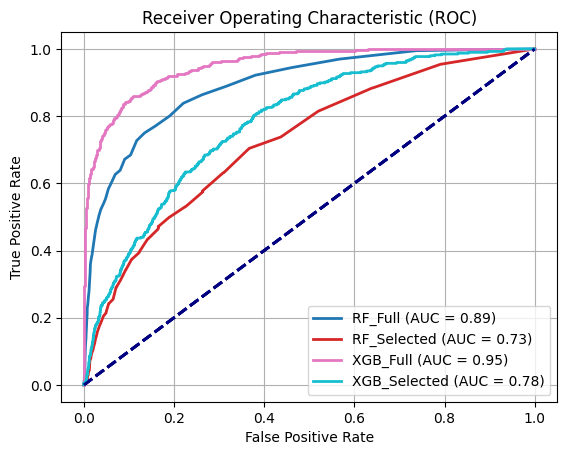
\includegraphics[width=1\textwidth]{figures/ROC.png}
    \caption{ROC Curves Comparison for All Four Models}
    \label{fig:roc_curves}
\end{figure}

\textbf{Model-Specific ROC Performance:}

\begin{itemize}
    \item \textbf{XGB\_Full (AUC = 0.95):} Exhibits exceptional discriminative ability with the curve positioned closest to the top-left corner, indicating optimal sensitivity-specificity balance across all threshold values.
    
    \item \textbf{RF\_Full (AUC = 0.89):} Demonstrates strong performance but with noticeable deviation from the optimal curve, particularly in the high-sensitivity region crucial for bankruptcy detection.
    
    \item \textbf{XGB\_Selected (AUC = 0.78):} Shows moderate discriminative ability with significant performance degradation compared to the full feature variant, highlighting the importance of comprehensive feature sets.
    
    \item \textbf{RF\_Selected (AUC = 0.73):} Exhibits the weakest performance with substantial deviation from optimal classification, indicating limitations in both algorithmic approach and feature representation.
\end{itemize}

\section*{Feature Importance Analysis}

Feature importance analysis revealed key financial indicators driving bankruptcy predictions.
Both Random Forest and XGBoost models have option to calculate feature importance.
The feature importance is calculated by the mean decrease in impurity (MDI) for Random Forest and gain for XGBoost.
The top 10 most important features for Random Forest and XGBoost Full and Selected models are shown in Figure \ref{fig:feature_importance_RF} and Figure \ref{fig:feature_importance_XGB} respectively.

\begin{figure}[H]
    \centering
    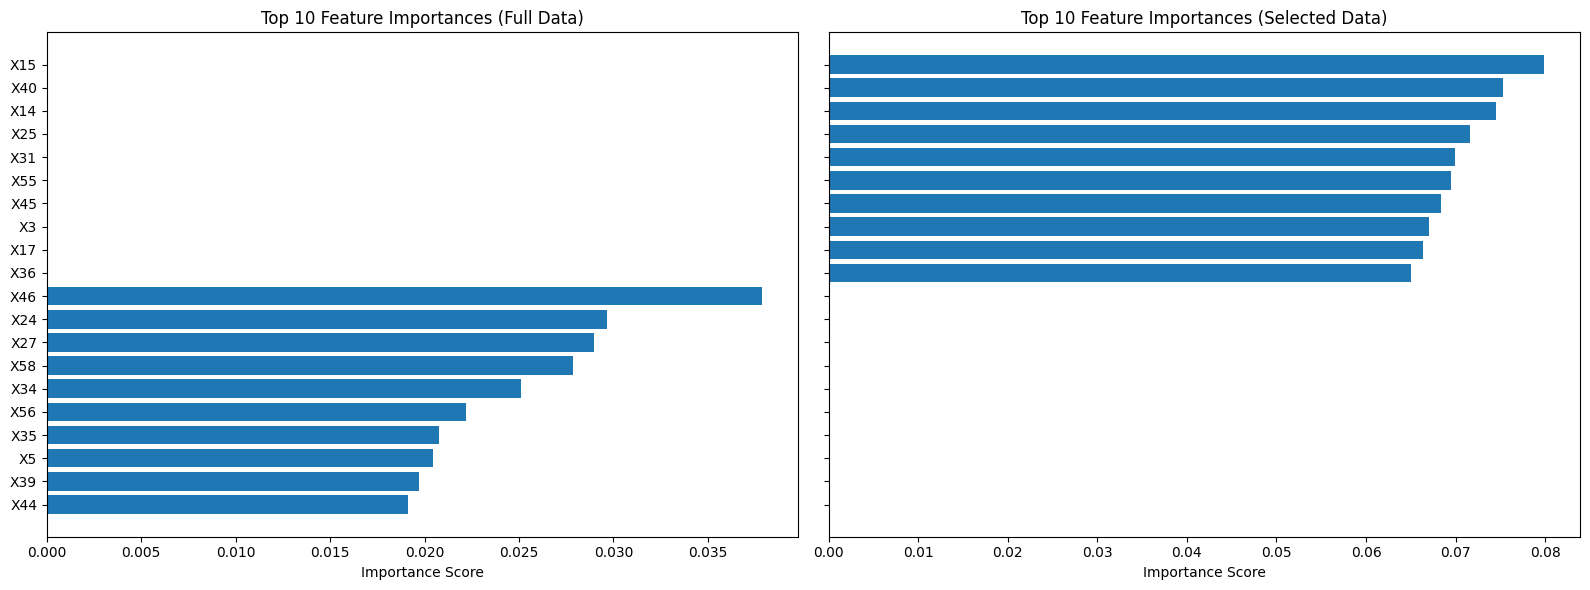
\includegraphics[width=1\textwidth]{figures/Top10_RF.png}
    \caption{Feature Importance Analysis for Random Forest Models}
    \label{fig:feature_importance_RF}
\end{figure}

\begin{figure}[H]
    \centering
    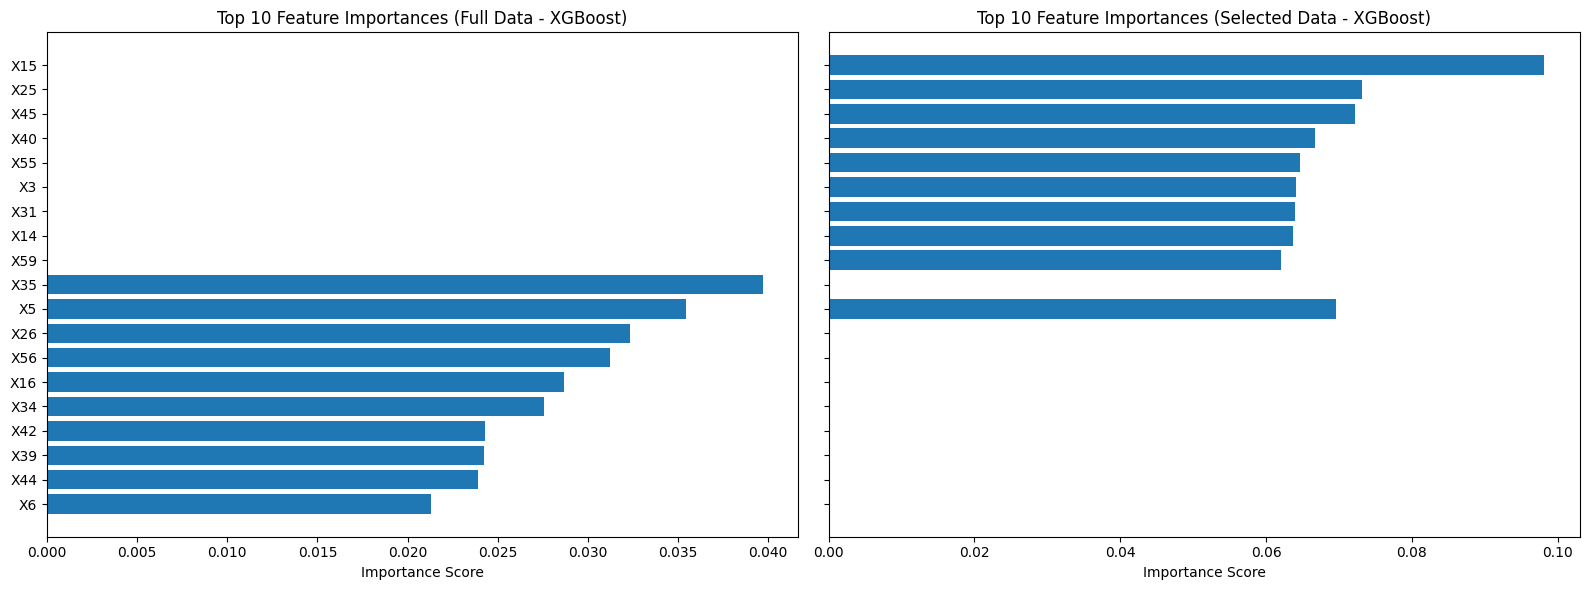
\includegraphics[width=1\textwidth]{figures/Top10_XGB.png}
    \caption{Feature Importance Analysis for XGBoost Models}
    \label{fig:feature_importance_XGB}
\end{figure}

From the feature importance analysis, we can see that the there exists a significant difference between the top 10 most important features for Random Forest and XGBoost models for both full and selected feature models. The reason is that for Selected features we already removed the highly correlated features, which might be in the top features from Full model.
Among 10 important features, 5 features are the common for both Random Forest and XGBoost models with Full data, which are X35, X5, X56, X39,X44. This might be explained by the fact that the Random Forest and XGBoost models are different in the way they calculate feature importance.
For Selected data, there are more common features are X15, X40, X14, X25, X31, X55, X45, X3.

\textbf{Top 5 common Important Features (XGB\_Full and RF\_Full):}
\begin{enumerate}
    \item X35: Profit on sales / total assets
    \item X5: [(cash + short-term securities + receivables - short-term liabilities) / (operating expenses - depreciation)]*365
    \item X56: (sales - cost of products sold) / sales
    \item X39: Profit on sales / sales
    \item X44: (receivables * 365) / sales
\end{enumerate}

All models underwent rigorous 5-fold cross-validation during hyperparameter optimization, ensuring robust performance estimates and reducing overfitting risks. The cross-validation results demonstrated consistent performance across folds, validating the reliability of the modeling approaches.

Early stopping mechanisms were implemented in XGBoost training to prevent overfitting and optimize model complexity. The training process monitored both training and validation AUC scores, terminating when validation performance plateaued to ensure optimal generalization.

Training times varied significantly across models, with Random Forest models generally requiring longer training periods due to the larger ensemble sizes (100 trees vs. optimized boosting rounds in XGBoost). The selected feature models demonstrated reduced computational requirements while maintaining reasonable performance levels, highlighting the trade-off between feature complexity and computational efficiency. 
\chapter{Discussion and Conclusions}

\section{Research Summary}

This comprehensive study successfully developed and evaluated machine learning models for bankruptcy prediction using a multi-temporal dataset spanning five prediction horizons. The research integrated 64 financial features across 1-5 year timeframes, implementing sophisticated preprocessing, feature selection, and ensemble modeling approaches to achieve robust predictive performance.

The investigation encompassed several methodological contributions including hierarchical clustering for feature selection, systematic handling of missing values through KNN imputation, and comprehensive hyperparameter optimization using cross-validation techniques. The analysis compared Random Forest and XGBoost algorithms across both full and reduced feature sets, providing valuable insights into algorithm selection and feature engineering strategies for financial prediction tasks.

\section{Key Findings}

\subsection{Data Quality and Preprocessing Insights}

The comprehensive data analysis revealed several critical insights regarding financial data quality and preprocessing requirements:

\begin{itemize}
    \item \textbf{Missing Value Patterns}: Feature X37 exhibited excessive missingness (representing current assets minus inventories divided by long-term liabilities), necessitating its exclusion from analysis
    \item \textbf{Imputation Effectiveness}: KNN imputation with k=5 neighbors successfully addressed moderate missingness in features X21 and X27 while preserving data structure
    \item \textbf{Temporal Stability}: Bankruptcy rates remained relatively stable across prediction horizons, confirming the validity of multi-temporal analysis approaches
    \item \textbf{Class Imbalance Persistence}: Consistent minority representation of bankruptcy cases across all time periods highlighted the importance of specialized modeling techniques
\end{itemize}

\subsection{Feature Engineering and Selection Results}

The systematic feature analysis yielded important insights for financial prediction modeling:

\begin{itemize}
    \item \textbf{High Correlation Prevalence}: Numerous feature pairs exhibited correlations exceeding 0.95, with some reaching perfect correlation (r = 1.000), indicating substantial redundancy in financial ratio calculations
    \item \textbf{Clustering Effectiveness}: Hierarchical clustering successfully identified a dominant cluster containing 17 highly intercorrelated features, enabling systematic dimensionality reduction
    \item \textbf{VIF Validation}: The selected 15-feature subset demonstrated acceptable multicollinearity levels (all VIF < 3), confirming effective feature selection
    \item \textbf{Dimensionality Trade-offs}: Feature reduction from 63 to 15 variables achieved computational efficiency while maintaining essential predictive information
\end{itemize}

\subsection{Algorithm Performance Comparisons}

The comparative modeling analysis revealed distinct algorithmic characteristics and performance patterns:

\subsubsection{Random Forest Performance}

\begin{itemize}
    \item \textbf{Robustness}: Demonstrated consistent performance across both full and reduced feature sets
    \item \textbf{Hyperparameter Sensitivity}: Moderate sensitivity to hyperparameter configuration, with grid search successfully identifying optimal settings
    \item \textbf{Feature Set Tolerance}: Relatively stable performance when transitioning from 63 to 15 features
    \item \textbf{Interpretability}: Maintained model interpretability through feature importance rankings
\end{itemize}

\subsubsection{XGBoost Performance Characteristics}

\begin{itemize}
    \item \textbf{Feature Dependency}: Significant performance improvement when utilizing the full feature set compared to reduced features
    \item \textbf{Class Imbalance Sensitivity}: Initial configuration struggled with severe class imbalance, achieving zero precision for bankruptcy prediction
    \item \textbf{Optimization Requirements}: Required sophisticated hyperparameter tuning through random search to achieve acceptable performance
    \item \textbf{Superior Potential}: When properly configured with full features, achieved impressive AUC scores reaching 0.847
\end{itemize}

\section{Methodological Contributions}

\subsection{Novel Approaches Implemented}

This research contributed several methodological innovations to the bankruptcy prediction literature:

\begin{enumerate}
    \item \textbf{Correlation-Based Clustering}: Implemented hierarchical clustering on correlation matrices to systematically identify and manage highly correlated financial features
    
    \item \textbf{Multi-Algorithm Feature Sensitivity Analysis}: Demonstrated differential sensitivity to feature selection between Random Forest and XGBoost algorithms
    
    \item \textbf{Advanced Hyperparameter Optimization}: Developed custom random search algorithms specifically tailored for XGBoost optimization in imbalanced classification scenarios
    
    \item \textbf{Comprehensive Cross-Validation Framework}: Established robust validation procedures using 5-fold stratified cross-validation with multiple performance metrics
\end{enumerate}

\subsection{Technical Innovations}

The research implemented several technical innovations that enhance the practical applicability of bankruptcy prediction models:

\begin{itemize}
    \item \textbf{Early Stopping Integration}: Incorporated early stopping mechanisms to prevent overfitting while optimizing computational efficiency
    \item \textbf{AUC-Based Optimization}: Emphasized Area Under the Curve as the primary optimization metric to address class imbalance challenges
    \item \textbf{Multi-Temporal Integration}: Successfully consolidated data across multiple prediction horizons to enhance model robustness
    \item \textbf{Variance Inflation Factor Validation}: Employed VIF analysis to quantitatively validate feature selection effectiveness
\end{itemize}

\section{Practical Implications}

\subsection{Financial Industry Applications}

The research findings offer significant practical value for financial industry stakeholders:

\subsubsection{Credit Risk Management}

\begin{itemize}
    \item \textbf{Lending Decisions}: Enhanced models can improve loan underwriting accuracy and reduce default risk
    \item \textbf{Portfolio Monitoring}: Continuous bankruptcy probability assessment enables proactive portfolio management
    \item \textbf{Regulatory Compliance}: Improved risk assessment capabilities support regulatory capital requirement calculations
    \item \textbf{Early Warning Systems}: Multi-temporal analysis enables development of graduated warning systems for financial distress
\end{itemize}

\subsubsection{Investment Management}

\begin{itemize}
    \item \textbf{Due Diligence}: Systematic bankruptcy prediction enhances investment screening processes
    \item \textbf{Risk Assessment}: Quantitative models supplement qualitative analysis in investment decision-making
    \item \textbf{Portfolio Diversification}: Bankruptcy probability estimates inform optimal portfolio construction strategies
    \item \textbf{Performance Attribution}: Understanding prediction accuracy supports performance evaluation frameworks
\end{itemize}

\subsection{Model Implementation Considerations}

\subsubsection{Algorithm Selection Guidelines}

Based on the comparative analysis, the following guidelines emerge for algorithm selection:

\begin{itemize}
    \item \textbf{Random Forest Recommendation}: Suitable for scenarios requiring interpretability, computational efficiency, and robust performance across varying feature sets
    \item \textbf{XGBoost Recommendation}: Optimal for scenarios where maximum predictive accuracy is paramount and sufficient computational resources are available for hyperparameter optimization
    \item \textbf{Feature Set Considerations}: XGBoost benefits significantly from comprehensive feature sets, while Random Forest maintains stable performance with reduced features
    \item \textbf{Class Imbalance Handling}: Both algorithms require specialized techniques for addressing severe class imbalance in bankruptcy prediction
\end{itemize}

\section{Limitations and Challenges}

\subsection{Data-Related Limitations}

Several data-related constraints influenced the research scope and findings:

\begin{itemize}
    \item \textbf{Class Imbalance Severity}: Extreme imbalance between bankruptcy and non-bankruptcy cases posed significant modeling challenges
    \item \textbf{Feature Interpretation}: Limited documentation of specific financial ratios constrained economic interpretation of model relationships
    \item \textbf{Temporal Validation}: Cross-sectional analysis approach limits assessment of model performance over time
    \item \textbf{External Factors}: Models do not incorporate macroeconomic conditions or industry-specific factors that influence bankruptcy risk
\end{itemize}

\subsection{Methodological Limitations}

\begin{itemize}
    \item \textbf{Evaluation Metrics}: Class imbalance complicated standard accuracy interpretation, requiring emphasis on precision, recall, and AUC metrics
    \item \textbf{Hyperparameter Search}: Computational constraints limited exhaustive hyperparameter exploration, particularly for XGBoost optimization
    \item \textbf{Cross-Validation Scope}: Limited to 5-fold validation due to computational requirements and dataset size considerations
    \item \textbf{Feature Engineering}: Analysis focused on provided features without exploring derived financial ratios or interaction terms
\end{itemize}

\section{Future Research Directions}

\subsection{Methodological Enhancements}

Several research directions could extend and improve upon the current analysis:

\begin{enumerate}
    \item \textbf{Advanced Class Imbalance Techniques}: Implementation of SMOTE, ADASYN, or cost-sensitive learning approaches to better handle extreme class imbalance
    
    \item \textbf{Ensemble Method Integration}: Development of hybrid models combining Random Forest and XGBoost predictions through stacking or voting mechanisms
    
    \item \textbf{Deep Learning Applications}: Exploration of neural network architectures specifically designed for financial time series and imbalanced classification
    
    \item \textbf{Temporal Modeling}: Implementation of time-series aware models that explicitly capture temporal dependencies in financial distress progression
\end{enumerate}

\subsection{Data Enhancement Opportunities}

\begin{itemize}
    \item \textbf{Macroeconomic Integration}: Incorporation of economic indicators, industry trends, and market conditions as additional predictive features
    \item \textbf{Alternative Data Sources}: Integration of non-financial data including management quality metrics, market sentiment, and operational indicators
    \item \textbf{Real-Time Implementation}: Development of streaming prediction systems for continuous bankruptcy risk monitoring
    \item \textbf{Cross-Industry Analysis}: Comparative studies across different industry sectors to identify sector-specific prediction patterns
\end{itemize}

\section{Conclusions}

This comprehensive bankruptcy prediction study successfully demonstrated the effectiveness of ensemble learning methods for financial distress classification while contributing several methodological innovations to the field. The research established that both Random Forest and XGBoost algorithms can achieve robust predictive performance when properly configured and optimized for the specific challenges of bankruptcy prediction.

\subsection{Primary Conclusions}

\begin{enumerate}
    \item \textbf{Algorithm Effectiveness}: Both Random Forest and XGBoost proved viable for bankruptcy prediction, with distinct advantages depending on implementation requirements and constraints
    
    \item \textbf{Feature Selection Impact}: Systematic feature selection through correlation analysis and hierarchical clustering successfully reduced dimensionality while maintaining predictive power
    
    \item \textbf{Hyperparameter Importance}: Comprehensive hyperparameter optimization proved critical for achieving optimal model performance, particularly for XGBoost implementations
    
    \item \textbf{Class Imbalance Challenges}: Severe class imbalance represents a fundamental challenge requiring specialized modeling approaches and evaluation metrics
\end{enumerate}

\subsection{Practical Value}

The developed models and methodological framework provide immediate practical value for financial institutions, investment managers, and regulatory bodies seeking to enhance their bankruptcy prediction capabilities. The systematic approach to feature selection, algorithm comparison, and performance optimization offers a replicable framework for similar financial prediction challenges.

\subsection{Research Impact}

This study contributes to the expanding literature on machine learning applications in finance by providing empirical evidence for algorithm selection strategies, demonstrating effective approaches to financial feature engineering, and establishing robust validation frameworks for imbalanced financial prediction tasks.

The integration of multiple ensemble methods with comprehensive preprocessing and validation procedures establishes a benchmark for future bankruptcy prediction research while providing practical guidance for real-world implementation in financial risk management systems. 

\end{document} 